\documentclass[12pt]{article}
\usepackage[top=1in, bottom=1in, left=.75in, right=.75in]{geometry}
\usepackage{amsmath}
%\usepackage[shortlabels]{enumitem}
\usepackage{enumerate}
\usepackage{fancyhdr}
\usepackage{graphicx, xcolor, setspace}
\usepackage{txfonts}
\usepackage{multicol,coordsys,pgfplots}
\usepackage[scaled=0.86]{helvet}
\renewcommand{\emph}[1]{\textsf{\textbf{#1}}}
\usepackage{anyfontsize}
% \usepackage{times}
% \usepackage[lf]{MinionPro}
\usepackage{tikz,pgfplots}
%\def\degC{{}^\circ{\rm C}}
\def\ra{\rightarrow}
\usetikzlibrary{calc,arrows.meta, shapes}
\pgfplotsset{compat = newest}
\newcommand{\blank}[1]{\rule{#1}{0.75pt}}

\pgfplotsset{my style/.append style={axis x line=middle, axis y line=
middle, xlabel={$x$}, ylabel={$y$}}}

%axis equal

%yticklabels={,,} , xticklabels={,,}

% \setmainfont{Times}
% \def\sansfont{Lucida Grande Bold}
\parindent 0pt
\parskip 4pt
\pagestyle{fancy}
\fancyfoot[C]{\emph{\thepage}}
\fancyfoot[R]{v1}
\fancyhead[L]{\ifnum \value{page} > 1\relax\emph{Math F251X Calculus I: Midterm 2}\fi}
\fancyhead[R]{\ifnum \value{page} > 1\relax\emph{Fall 2023}\fi}
\headheight 15pt
\renewcommand{\headrulewidth}{0pt}
\renewcommand{\footrulewidth}{0pt}
\let\ds\displaystyle
\def\continued{{\emph {Continued....}}}
\def\continuing{{\emph {Problem \arabic{probcount} continued....}}\par\vskip 4pt}


\newcounter{probcount}
\newcounter{subprobcount}
\newcommand{\thesubproblem}{\emph{\alph{subprobcount}.}}
\def\problem#1{\setcounter{subprobcount}{0}%
\addtocounter{probcount}{1}{\emph{\arabic{probcount}.\hskip 1em(#1)}}\par}
\def\subproblem#1{\par\hangindent=1em\hangafter=0{%
\addtocounter{subprobcount}{1}\thesubproblem\emph{#1}\hskip 1em}}
\def\probskip{\vskip 10pt}
\def\medprobskip{\vskip 2in}
\def\subprobskip{\vskip 45pt}
\def\bigprobskip{\vskip 4in}


\newenvironment{subproblems}{%
\begin{enumerate}%
\setcounter{enumi}{\value{subprobcount}}%
\renewcommand{\theenumi}{\emph{\alph{enumi}}}}%
{\setcounter{subprobcount}{\value{enumi}}\end{enumerate}}


\newcommand{\be}{\begin{enumerate}}
\newcommand{\ee}{\end{enumerate}}


\begin{document}

{\emph{\fontsize{26}{28}\selectfont Fall 2023 \hfill
\hfill Math F251X}}

\begin{center}
{\emph{\fontsize{32}{36}\selectfont Calculus I: Midterm 2}}
\end{center}
\vskip 1.cm
\strut\vtop{\halign{\emph#\hskip 0.5em\hfil&#\hbox to 2in{\hrulefill}\cr
\emph{\fontsize{18}{22}\selectfont Name:}&\cr
\noalign{\vskip 10pt}
%\emph{\fontsize{18}{22}\selectfont Student Id:}&\cr
%\noalign{\vskip 10pt}
%\emph{\fontsize{18}{22}\selectfont Calculator Model:}&\cr
}}
%\hfill
%\vtop{\halign{\emph{\fontsize{18}{22}\selectfont #}\hfil& \emph{\fontsize{18}{22}\selectfont\hskip 0.5ex $\square$ #}\hfil\cr
%Section: & 001 (Jill Faudree)\cr
%\noalign{\vskip 4pt}
%         & 002 (Ryan Bridges)\cr
%\noalign{\vskip 4pt}
%         & 005 (Leah Berman)\cr}}
%
\vfill
{\fontsize{18}{22}\selectfont\emph{Rules:}}

\begin{itemize}
\item Partial credit will be awarded, but you must {\bf show your work}.

\item You may have a single handwritten $3'' \times 5''$ notecard, both sides.

\item Calculators are \emph{not allowed}. 

\item Place a box around your  \fbox{FINAL ANSWER} to each question where appropriate.

\item Turn off anything that might go beep during the exam.

\end{itemize}

%If you need extra space, you can use the back sides of the pages.
%Please make it obvious  when you have done so.



Good luck!
\vfill
\def\emptybox{\hbox to 2em{\vrule height 16pt depth 8pt width 0pt\hfil}}
\def\tline{\noalign{\hrule}}
\centerline{\vbox{\offinterlineskip
{
\bf\sf\fontsize{18pt}{22pt}\selectfont
\hrule
\halign{
\vrule#&\strut\quad\hfil#\hfil\quad&\vrule#&\quad\hfil#\hfil\quad
&\vrule#&\quad\hfil#\hfil\quad&\vrule#\cr
height 3pt&\omit&&\omit&&\omit&\cr
&Problem&&Possible&&Score&\cr\tline
height 3pt&\omit&&\omit&&\omit&\cr
&1&&8&&\emptybox&\cr\tline
&2&&7&&\emptybox&\cr\tline
&3&&18&&\emptybox&\cr\tline
&4&&11&&\emptybox&\cr\tline
&5&&12&&\emptybox&\cr\tline
&6&&12&&\emptybox&\cr\tline
&7&&10&&\emptybox&\cr\tline
&8&&12&&\emptybox&\cr\tline
&9&&10&&\emptybox&\cr\tline \tline
&Extra Credit&&5&&\emptybox&\cr\tline
&Total&&100&&\emptybox&\cr
}\hrule}}}

\newpage
%\begin{enumerate}
%%%%


%%%%%%%% Linear Approximation
\problem{8 points} Consider the function $f(x)  = \sqrt[3]{x}$.


\begin{subproblems}
\item  Determine the \emph{linear approximation} $L(x)$ of the function at the point $a=64 = 4^{3}$.
\vfill
\item  Use the linear approximation you just found to \emph{estimate} $\displaystyle{ \sqrt[3]{70}}$.% Give your answer as a fraction.
\vfill
\end{subproblems}

%%%%%%%%%%% critical points and extreme value theorem
\problem{7 points} Consider the function \[\displaystyle{ j(t) = \cos(t) + (\sin(t))^{2} }.\]
%\begin{subproblems}
%\item Find all critical values of  $j(t)$  in the interval $\displaystyle{ [0, 2\pi]}$.
%
%\vfill
%
%\item 
Determine the \emph{absolute minimum} and \emph{absolute maximum} values of $j(t)$ on the interval
$\displaystyle{ [0, \pi]}$. Show your work.

% and the $t$-values in the interval $[0, \pi]$ where these absolute maximum and minimum values occur.
\vfill

Absolute maximum: \blank{1in}

%$t$-value(s) in $[0,\pi]$ where the absolute maximum occurs:  \blank{1in}

Absolute minimum: \blank{1in}

%$t$-value(s)in $[0,\pi]$ where the absolute minimum occurs:  \blank{1in}
%\end{subproblems}

\newpage

%%%%%% 
%%%%%%%%% curve analysis, algebraically
\problem{18 points} 
Answer the questions below about the function $\ds f(x)=\frac{x^{4}}{e^x}.$ It is a fact that after simplification, \[ \quad f'(x)=\frac{ -x^3(x-4)}{e^{x}}, \quad \text{ and }  f''(x)=\frac{ x^2(x-6)(x-2)}{e^x}\]
You must show your work and justify your conclusion with a few words or a computation. Make sure someone else can follow your work.
\begin{subproblems}
	\item Determine the intervals where $f$ is \emph{increasing} and where $f$ is \emph{decreasing}. Show your work.
	\vfill
	
	
	
	%Fill in the blanks: $f(x)$ is increasing on the interval \blank{1in}  and decreasing on the interval \blank{1in} . (If $f$ is never increasing or never decreasing, write ``none'' for that interval.)
	
	Increasing: \hrulefill Decreasing:\hrulefill	(If none write ``none''.)
	
	\item %Find the $x$-values of all {\bf local minima} and {\bf local maxima} of $f$. 
	%\vspace{.5in}
		Fill in the blanks: $f(x)$ has a local maximum at $x = $ \blank{1in}  and a local minimum at $x = \blank{1in} $. (If none, write ``none''.)
		
%		\hfill \emph{...continued on next page}
%		\newpage
%		
%		\emph{...continued from previous page}
%		
%		Recall
%		\[\ds f(x)=\frac{x^{4}}{e^x},\quad f'(x)=\frac{ -x^3(x-4)}{e^{x}}, \quad \text{ and }  f''(x)=\frac{ x^2(x-6)(x-2)}{e^x}.\]

	\item Find all intervals where $f$ is \emph{concave up} and where $f$ is \emph{concave down}. Show your work.
	\vfill
	%Fill in the blanks: $f(x)$ is concave up on the interval \blank{1in}  and concave down on the interval \blank{1in} . (If $f$ is never concave up or concave down, write ``none'' for that interval.)
	Concave up: \hrulefill Concave down:\hrulefill	(If none write ``none''.)
	
	\item %Find the {\bf $x$-values} of all {\bf inflection points} of $f$.
	%\vspace{.5in}
			Fill in the blanks: $f(x)$ has (an) inflection point(s) at $x =$ \blank{1in}. (If none, write ``none''.)
	%Fill in the blanks: $f(x)$ is concave up on the interval \blank{1in} 
%	and concave down on the interval \blank{1in} . (If $f$ is never concave up or concave down, write ``none'' for that interval.)	
	
%	\bigskip
%	
%	\item Evaluate the following limits and show your work clearly. An answer without work/justification may not receive credit. If you use L'H\^opital's rule, you \emph{must} indicate that by writing $\stackrel{H}{=}$ or $\stackrel{L'H}{=}$ or something similar.
%	\begin{subproblems}
%	\item $\ds \lim_{x\rightarrow \infty}f(x)$ =  
%	\vspace{1in}
%	
%	 \item $\ds \lim_{x\rightarrow -\infty}f(x)$ = 
%	 	\vspace{1in}
%	 \end{subproblems}
%	 
%	 	Write the \emph{equation} of the horizontal asymptote(s) of $f(x)$, if they exist. \blank{2in} If none exist, write ``none''. 
	\end{subproblems}
%

\newpage

%%%%%%%%% Curve sketching with concavity/increasing/decreasing/etc

\problem{11 points} \emph{Sketch} a graph of a function $h(x)$ that satisfies all of the following properties. 

After drawing the graph:

\begin{itemize}
\item \emph{Label} on the graph the following things, if they exist, by drawing a point on the graph and labeling: any local maximums by writing  \textsf{LOCAL MAX}, local minimums by writing \textsf{LOCAL MIN}, inflection points by writing \textsf{IP} 
\item Draw any horizontal and vertical asymptotes with dashed lines and \emph{label} them with their equation.
\item Mark any important $x$-values and $y$-values on the $x$- and $y$-axes.
\end{itemize}


\emph{Properties:}
\begin{multicols}{2}
\begin{itemize}
\item The domain of $h(x)$ is $(-\infty, \infty)$
\item $h(-2)=4$ and $h(2)=0$
\item $h'(x) > 0$ when $x < -2$
\item $h'(x) < 0$ when $x > -2$
\columnbreak
\item $h''(x) < 0$ when $x<0$
\item $h''(x) > 0$ when $x>0$
\item $\ds \lim_{x \to -\infty} h(x) = -\infty$
\item $\ds \lim_{x \to \infty} h(x) = -5$
\end{itemize}
\end{multicols}

\begin{tikzpicture}
\draw[<->] (-8,0) --  (8,0);
\draw[<->] (0,4) -- (0,-4);
\end{tikzpicture}
\newpage

%%%%%%%%%%%% Optimization

\problem{12 points} 
\begin{minipage}[b]{.6\linewidth}
An open box is to be constructed by cutting squares out of the four corners of a $3$ foot by $3$ foot piece of cardboard and folding up the sides. (See the diagram. Note that the box will not have a lid, and the height of the box will be $x$ feet.)
\end{minipage}
%
\hfill
%
\begin{minipage}{.3\linewidth}
\def\r{.4}
\begin{tikzpicture}[scale=1]
\def\xx{3}
\def\yy{3}

\draw[fill = gray!50] (0,0) rectangle (\r, \r);
\draw[fill = gray!50] (\xx,\yy) rectangle (\xx-\r, \yy-\r);
\draw[fill = gray!50] (\xx,0) rectangle (\xx-\r, \r);
\draw[fill = gray!50] (0,\yy) rectangle (\r, \yy-\r);
\draw[ultra thick] (0,0) rectangle (\xx,\yy);
\draw (\xx-\r, \r/2) node[left] {$x$};
\draw (\xx-\r/2, \r) node[above] {$x$};
\draw (\r, \r/2) node[right] {$x$};
\draw (\r/2, \r) node[above] {$x$};
\draw (\r, \yy-\r/2) node[right] {$x$};
\draw (\xx-\r/2, \yy-\r) node[below] {$x$};
\draw (\r/2, \yy-\r) node[below] {$x$};
\draw (\xx-\r, \yy-\r/2) node[left] {$x$};
%\draw[|-|] (4-\r-.2, \r) -- node[midway, fill = white, inner sep = 2] {$x$} (4-\r-.2, .02);
%\draw[|-|] (4-\r, \r+.2) -- node[midway, fill = white, inner sep = 2] {$x$} (4, \r+.2);
%\draw[|-|] (0, \r+.2) -- node[midway, fill = white, inner sep = 2] {$x$} (\r, \r+.2);
%\draw[|-|] (\r + .2, 0) -- node[midway, fill = white, inner sep = 2] {$x$} (\r+.2, \r);
%\draw[|-|] (0 , 2-\r- .2) -- node[midway, fill = white, inner sep = 2] {$x$} (\r, 2-\r-.2);
%\draw[|-|] (4-\r , 2-\r- .2) -- node[midway, fill = white, inner sep = 2] {$x$} (4, 2-\r-.2);
%\draw[thick,|-|] (4-\r-.2 , 2-\r) -- node[midway, fill = white, inner sep = 2] {$x$} (4-\r-.2, 2);
%\draw[|-|] (\r+.2 , 2-\r) -- node[midway, fill = white, inner sep = 2] {$x$} (\r+.2, 2);
\draw[|-|](0,-.3) -- node[ midway, fill = white, inner sep = 2] {$\xx$ ft} (\xx, -.3);
\draw[|-|](\xx+.3,0) -- node[right, fill = white, inner sep = 2] {$\yy$ ft} (\xx+.3, \yy);
\draw[dashed] (\r,\r) rectangle (\xx-\r, \yy-\r);
\end{tikzpicture}
\end{minipage}

%\includegraphics[scale=0.6]{boxpic}
\begin{subproblems}
\item Write an equation for the \emph{volume} of the box in terms of the variable $x$.
\vspace{1in}
\item %Determine which $x$ will {\bf maximize the volume} of the box. 
Determine the \emph{dimensions} of the box with the largest volume.
Show your work, and use calculus to \emph{justify} that your answer is the maximum. Include units in your final answer. An answer with no clear justification will not receive full credit.

\vfill

\vfill

\vfill

Dimensions: length: \blank{1in} width: \blank{1in} height: \blank{1in}

\end{subproblems}

\newpage

%%%%%%%%%%% Limits at infinity and indeterminate type and L'Hopital's rule

\problem{12 points} Evaluate the following limits. Show your work. If you use L'H\^opital's rule, you must indicate where you are using it by writing $\stackrel{H}{=}$ or $\stackrel{L'H}{=}$ or something similar.
\begin{subproblems}
\item $\ds \lim_{x \rightarrow 2} \frac{3^x-x^3-1}{x-2}$
\vfill
\item $\ds \lim_{x \rightarrow 0} \frac{x^2-x}{2\sin x - 2}$
\vfill
\item $\ds \lim_{x \rightarrow \infty} \frac{\ln x}{\sqrt{x}}$
\vfill
\item $\ds \lim_{x \rightarrow \infty} xe^{-x}$
\vfill
\end{subproblems}

\newpage
%%%%%%%%%%% related rates %%%%%%%
\problem{10 points} 
\begin{minipage}{.8\textwidth}A giant ice cylinder, being prepared for the World Ice Art Championships, is carved to have a radius of 100 cm and a height of 300 cm. The cylinder is uniformly melting, which means that the ratio of the radius to the height remains constant: specifically, $\frac{r}{h}= \frac{1}{3}$. If the height is \emph{decreasing} at a rate of $2$ cm/hour, how fast is the surface area changing when the cylinder is $150$ cm tall? 

\bigskip

Write your answer in a complete sentence, using units.

\bigskip

Recall that the surface area of a cylinder with radius $r$ and height $h$ is $\displaystyle{S= 2\pi r h + 2\pi r^2.}$ %answer the following questions. %Answer the following question when $r= 2 m$ and $h = 3 m$. 
\end{minipage}
% Note that the volume of a cylinder is calculated as $\displaystyle{V = \pi r^3 h}$ and the surface area of a cylinder is calculated as $\displaystyle{S= 2\pi r h + 2\pi r^2.}$ 
\hfill
\begin{minipage}{.2\textwidth}
\begin{center}
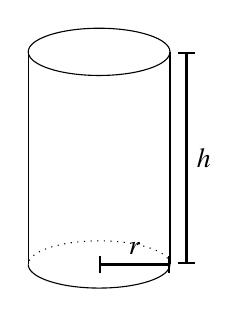
\begin{tikzpicture}[scale = .3]
\draw (3,0) arc (0:360: 3 and 1);
\draw (-3,-9) arc (180:360: 3 and 1);
\draw[dotted] (3,-9) arc (0:180: 3 and 1);
\draw (3,0) -- (3,-9);
\draw (-3,0) -- (-3,-9);
\draw[|-|, thick] (0,-9) -- node[above]{$r$} (3,-9) ;
\draw[|-|, thick] (3.7,-9) -- node[right]{$h$} (3.7,0) ;

%  \node (a) [cylinder, shape border rotate=90, draw, minimum height=15mm, minimum width=7.5mm] {};
%  \draw [<->] ([xshift=5pt]a.before bottom) -- ([xshift=5pt]a.after top) node [midway, right] {$h$};
%  
%  \draw [<->] ([yshift=-5pt]a.top) -- ([yshift=-5pt]a.top -| a.before top) node [midway, above] {$r$};
\end{tikzpicture}
\end{center}
\end{minipage}
%\begin{subproblems}
%\item [$(a)$] $\displaystyle{\frac{dV}{dt}}$
%\item How fast is the volume changing when the radius of the cylinder is $1/2$ meter (50 cm)?
%\vfill

%\item [$(b)$] $\displaystyle{\frac{dS}{dt}}$
%\vfill How fast is the surface area changing when the radius of the cylinder is $1/2$ meter (50 cm)?

%\vfill

%\item [$(c)$] $\displaystyle{\frac{dS}{dV}}$
%\vfill
% 
%\end{subproblems}

\newpage

%%%%%%%%%

%%%%%%%%%% section 5.1 and 5.2, definite integrals and riemann sums


\problem{12 points} A portion of the function \[f(x) = \begin{cases} \sqrt{25-x^{2}} \quad -5 \leq x \leq 5 \\ -\frac{1}{2}(x-5) \quad x \geq 5
\end{cases} \]
is graphed below.

\begin{center}
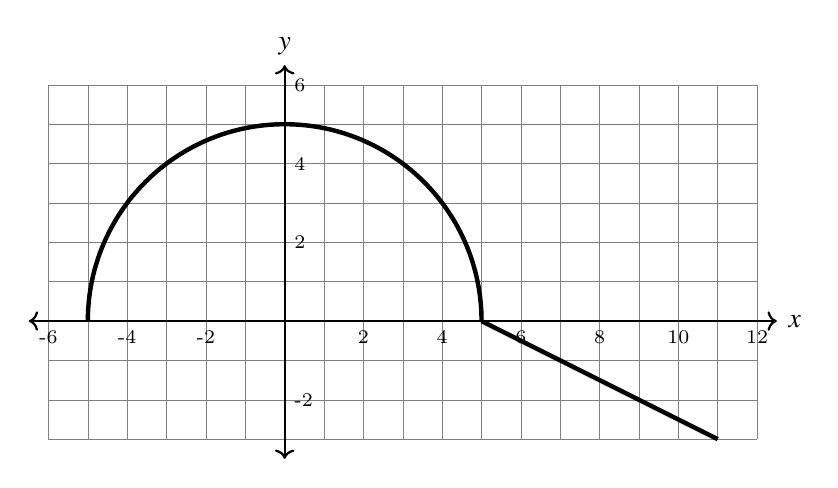
\begin{tikzpicture}[scale = .5]
%cubic
%\begin{axis}[xscale = 1, yscale = 1, thick, my style, xtick={-2,2,4,...,10}, ytick={-1,1,2,3,4},xmin=-5, xmax=10, ymin=-5, ymax=6, minor y tick num=1, minor x tick num=1, 
%mark size=3.0pt, grid = major, ]
%%\addplot[ultra thick, -,domain=-4:-2, samples=100, <-]coordinates {(-4,-2)(-2,2)};
%\addplot[ultra thick, domain=-5:5, samples=100, ,]{sqrt(25-x^2)};
%\addplot[ultra thick, ->,domain=5:9, samples=100]{-1/2*(x-5)};
%\end{axis}

\draw[help lines] (-6, -3) grid (12, 6);
\draw[thick,<->] (-6.5,0) -- (12.5,0) node[right] {$x$};
\draw[thick,<->] (0,-3.5) -- (0,6.5) node[above] {$y$};
\draw[ultra thick] (5,0) -- (11,-3);
\draw[ultra thick] (5,0) arc (0:180:5);
\foreach \i in {-6, -4,-2,2,4,6,8,10, 12} {\path  (\i,0)node[below, font = \scriptsize] {\i};}
\foreach \i in {-2,2,4,6} {\path  (0, \i)node[right, font = \scriptsize] {\i};}

\end{tikzpicture}
\end{center}


\begin{subproblems}
\item We want to approximate $\ds \int_{0}^{9} f(x) \ dx$ using \emph{three} right-hand rectangles.

\begin{enumerate}[i.]
%\begin{subproblems}
\item \emph{Draw} the three right-hand rectangles on the graph. Lightly shade them in. Make sure I can tell where your rectangles are and try to be reasonably precise.
\bigskip

\item Now \emph{approximate} $\ds \int_{0}^{9} f(x) \ dx$ using the  three right-hand rectangles. (Your answer should be a number.)
\vfill

%\end{subproblems}
\end{enumerate}
\item Use geometry to compute $\ds \int_{0}^{9} f(x) \ dx$ exactly. Show your work.
\vfill

	\end{subproblems}


\newpage



%%%%%%%%% Antiderivatives
\problem{10 points} 
 
\begin{subproblems}

\item  Determine $H(\theta) = \ds \int \theta^{2/3} + (\sec(\theta))^{2} + 5 \ d\theta$. (Give the most generic answer.)
\vfill

\item  Determine $G(x) = \ds \int \frac{14x^{3}+2x +1}{x^{3}} \ dx$. (Give the most generic answer.)
\vfill
\item   Find two different antiderivatives for the function  $f(t) = \ds 4 e^{t} + \frac{1}{t}$.

\vfill



%\item   Determine whether the function $F(x) = \frac{1}{3}\left(\sqrt{x^{2} - 1}\right)^{3} + 12$ is an antiderivative for the function $f(x) = \sqrt{x^{2} - 1}$. Explain your answer.
%
%\vfill
\end{subproblems}

%\problem{6 points} A car is traveling at a velocity of 50 miles/hour ( = 4400 feet/second) when the brakes are applied, producing a constant negative acceleration (that is, deceleration) of $-22$ feet/second$^{2}$. How long does it take for the car to stop?
%\vfill
%
%\vfill
%\vfill




\newpage





%\end{enumerate}
%%%%%%%%%%%%%%%%%%%%%%%%%%%

\fbox{Extra Credit} (5 points) 
The left-hand graph shows the \fbox{DERIVATIVE} $k'$ of some function $k$.


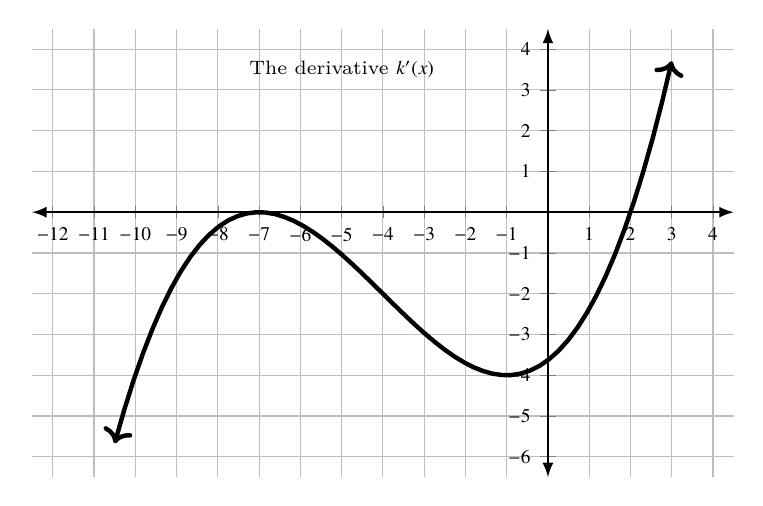
\begin{tikzpicture}
\begin{axis}[xscale = 1.3, yscale=1, %my style, 
xtick={-12,...,4}, ytick={-6,...,4},
xmin=-12.5, xmax=4.5, ymin=-6.5, ymax=4.5, minor y tick num=0,
minor x tick num=0, mark size=5.0pt,
grid=both, ylabel=$$,samples=60,
axis lines=middle,
axis line style={thick, latex-latex},font = \scriptsize
]
\addplot[domain=-10.5:3, <->, ultra thick] {-(-1/27*(x+7)^(2)*(x-2))};
% \addplot[only marks, mark size=2pt] coordinates {(0,-1.8) (7,2.4)};
\node at (axis cs:-5,3.5) [] {The derivative \ \\
	$k'(x)$}; %axis cs means ``axis coordinate system''
$$
\end{axis}
\end{tikzpicture}
\hfill
\begin{tikzpicture}[scale = 1]
\draw[<->] (-4,0) -- (4,0);
\draw[<->] (0,3) -- (0,-3);
%\path  (0,2.5) node [right]{draw $k(x)$ on these axes};
\end{tikzpicture}

\emph{The following questions are about the original function $k(x)$, \underline{not} the graphed $k'(x)$.}


\begin{enumerate}[a.]

%\item  Critical points of $k(x)$: \hrulefill 
%\vfill

%\vskip.2in

%\item  On what intervals is $k$ increasing or decreasing? 

%\vskip.1in

%Increasing: \hrulefill

%\vskip.1in

%Decreasing: \hrulefill

%\vskip.2in

%\vfill
\item At what value(s) of $x$ does $k$ have a local maximum or minimum? If none, say so. \emph{Write some words} to explain how you know that these $x$-values correspond to a local max or min (or not).

\vskip.2in

Local Max: $x = $ \hrulefill
Local Min: $x = $ \hrulefill

%\vskip.2in

%\item On what intervals is $k$ concave up or concave down? Use interval notation.\\

%Concave up: \hrulefill
%Concave down: \hrulefill

%\vskip.2in
\vfill

\item  At what values of $x$ does $k$ have inflection points? If none, say so. \emph{Write some words} to explain how you know that these $x$-values correspond to inflection points (or not).

\vskip.2in

Inflection points: $x = $ \hrulefill
\vfill

\item Sketch the graph of the original function $k(x)$ on the axes to the left of the derivative, using the fact that  $k(-7) = 1$. Your sketch does not have to be to scale, but it should show the right information regarding increasing/decreasing/max/min/concavity/inflection points. Mark important values on the $x-$ and $y$-axes.

\end{enumerate}




\end{document}

%%%%ENDDOCUMENT


